\ylDisplay{Allveelaev} % Ülesande nimi
{Mihkel Heidelberg} % Autor
{lahtine} % Voor
{2012} % Aasta
{G 5} % Ülesanne nr.
{6} % Raskustase
{
% Teema: Vedelike-mehaanika
\ifStatement
\begin{wrapfigure}{r}{0.51\linewidth}%
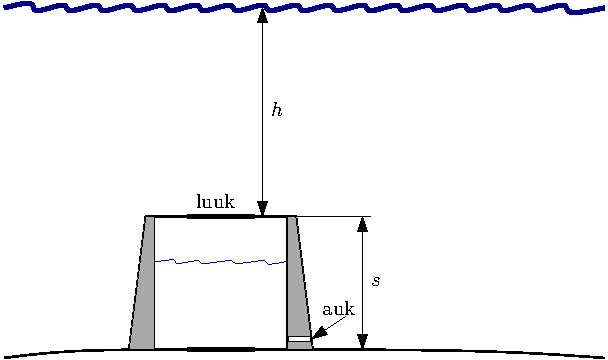
\includegraphics[width=\linewidth]{2012-lahg-05-allveelaev_g}%
\end{wrapfigure}
Salaagent Bond põgeneb allveelaevalt selle torni kaudu. Tornis on algselt
rõhk sama mis õhurõhk vee peal: $p_0 = \SI{100}{kPa}$. Pärast torni ja ülejäänud
allveelaeva eraldava luugi sulgemist teeb ta seina sisse augu (vaata joonist), misjärel
täitub torn osaliselt veega. Seejärel avab Bond torni laeluugi ja ujub
koos vabaneva õhuga pinnale.\\
\osa Kui paks on õhukiht, mis jääb torni enne torni
laeluugi avamist ja pärast vee sissevoolamise lõppemist?\\
\osa Kui suur ja mis suunas (üles või alla) on õhu ja vee poolt laeluugile avaldatav summaarne jõud enne
avamist, kui veetase torni sees on jäänud paigale?
\par
Luugi pindala $S =
\SI{0,50}{m^2}$, veetase luugi kohal $h=\SI{25}{m}$, torni kõrgus 
$s=\SI{2,0}{m}$. Vee tihedus $\rho = \SI{1000}{kg/m^3}$, raskuskiirendus $g =
\SI{9,8}{m/s^2}$.
\fi


\ifHint
\osa Vee sissevoolu lõppedes on hüdrostaatilised rõhud vees torni sees ja väljas tasakaalus. Õhurõhk torni sees vee kohal on võrdne hüdrostaatilise rõhuga samal tasemel tornist väljas.\\
\osa Luugile mõjub altpool torni sees oleva õhu rõhk ning ülevalt vee hüdrostaatiline rõhk.
\fi


\ifSolution
Vee sissevoolu lõppedes on hüdrostaatilised rõhud vees torni sees ja väljas tasakaalus, samuti on õhu temperatuur võrdsustunud vee omaga (vahepeal võib õhu temperatuur kokkusurumise tõttu veidi tõusta). Õhurõhk torni sees on võrdne hüdrostaatilise rõhuga tornis vee piiril. Rõhkude tasakaalust saame avaldada õhukihi paksuse:
$$ \rho g (h+d) + p_0 = p_0 \frac{s}{d},$$
$$ d^2 \rho g  + d (p_0 + h \rho g) - s p_0=0, $$
$$ d = \frac{( \pm \sqrt{(p_0 + h \rho g)^2 + 4 s \rho g p_0 } - p_0 - h \rho g)}{2\rho g }.$$
Lähteülesandele vastab positiivne lahend $d \approx \SI{57}{cm}$.
Kuna luugile mõjub altpoolt torni sees oleva õhu rõhk, mis vastab hüdrostaatilisele rõhule sügavusel $d+h$, saame, et summaarne jõud mõjub ülespoole:
$$F = A(\rho g (d+h) + p_0 - \rho g h - p_0) = A \rho g d \approx \SI{2800}{N}.  $$ 
Kui Bond torni vett sisse ei laseks, oleks vee ja õhu poolt summaarne luugile mõjuv jõud allapoole $A \rho g h \approx \SI{120}{kN}$. Eeldusel, et luuk avaneb väljapoole, seda inimjõul lahti ei saa.
\fi


\ifEngStatement
% Problem name: Submarine
\begin{wrapfigure}{r}{0.51\linewidth}%
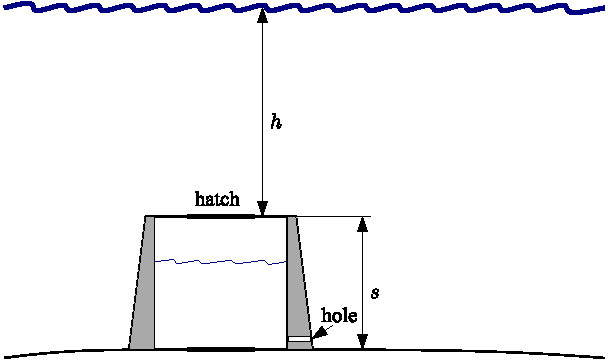
\includegraphics[width=\linewidth]{2012-lahg-05-allveelaev_g_ing}%
\end{wrapfigure}
Secret agent Bond is escaping from a submarine through its tower. Initially the pressure in the tower is the same as the air pressure on the water: $p_0 = \SI{100}{kPa}$. After closing the hatch that separates the tower from the rest of the submarine Bond makes a hole inside the tower’s wall (see figure), after which the tower partly fills with water. Next, Bond opens the ceiling hatch and swims to the surface with the released air.\\
a) How thick is the air layer that is inside the tower before opening the ceiling hatch and after the water has stopped flowing inside?\\
b) How big and to what direction (up or down) is the total force applied to the ceiling hatch by the air and the water before opening the hatch and during the time when the water level inside tower has stilled?\\
The area of the hatch is $S =
\SI{0,50}{m^2}$, the water level above the hatch $h=\SI{25}{m}$, the height of the tower $s=\SI{2,0}{m}$. The density of water $\rho = \SI{1000}{kg/m^3}$, gravitational acceleration $g =
\SI{9,8}{m/s^2}$.
\fi


\ifEngHint
a) When the inflow of water ends the hydrostatic pressures in water are the same inside and outside of the tower. The air pressure inside the tower above the water is equal to the hydrostatic pressure at the same level outside the tower.\\
b) Below the hatch the air pressure inside the tower is applied to it and above the hatch the hydrostatic pressure is applied.
\fi


\ifEngSolution
By the end of the water inflow the hydrostatic forces in the water are balanced inside the tower and outside, the air temperature has also gotten equal with the water’s temperature (the air temperature might rise a bit in between due to compression). The air pressure inside the tower is equal to the hydrostatic pressure in the tower at the water’s level. From the equilibrium of pressures we can express the air layer’s width:
$$ \rho g (h+d) + p_0 = p_0 \frac{s}{d},$$
$$ d^2 \rho g  + d (p_0 + h \rho g) - s p_0=0, $$
$$ d = \frac{( \pm \sqrt{(p_0 + h \rho g)^2 + 4 s \rho g p_0 } - p_0 - h \rho g)}{2\rho g }.$$
The positive solution $d \approx \SI{57}{cm}$ corresponds to our problem. Because the hatch is affected from below by the air pressure inside the tower that corresponds to the hydrostatic pressure at a depth $d+h$ we get that the following total force is applied upwards:
$$F = A(\rho g (d+h) + p_0 - \rho g h - p_0) = A \rho g d \approx \SI{2800}{N}.  $$
If Bond would not let water inside the tower then the total downwards force applied to the hatch by the water and the air would be $A \rho g h \approx \SI{120}{kN}$. Assuming that the hatch opens outwards no human force could open it.
\fi
}